\lab{Python}{Vectorization}{Vectorization}
\label{lab:Python_Vectorization}

In Python, the cost of looping over a sequence is sometime prohibitive.
One method for avoiding these explicit for-loops is to \emph{vectorize} our code.
NumPy allows operation that normally apply only to scalars to also work seamlessly with NumPy arrays.
Some of the benefits of allowing these types of operations are concise code and fast execution.

\section*{A Simple Example}
We explore the benefits of vectorization in calculating the squared Euclidean distance of a set of points.
This distance metric is commonly used in machine learning algorithms to calculate the how far apart data points lie from each other.
Being able to calculate these distances is essential in quickly calculating nearest neighbors and other spatial algorithms.
We start with a naive version.  Given two matrices, $A$ and $B$, it will calculate the squared Euclidean distance between points
represented as rows in both matrices.  The reason we calculate the squared distance instead of the true Euclidean distance is because
taking the square root of a number is time consuming.
\begin{lstlisting}
def slow_sqdist(A, B):
    m = A.shape[0]
    n = B.shape[0]
    
    E = np.zeros((m, n))
    for i in xrange(m):
        for j in xrange(n):
            E[i, j] = ((A[i] - B[j])**2).sum()
    return E
\end{lstlisting}
The naive version reasonably quickly for small sets of points.  However, increasing the number of points quickly slows down the algorithm.
The motivating idea of vectorization is make NumPy take care of the looping.  
We can easily vectorize the inner loop.  Instead of setting each element of E individually, we will calculate entire rows at a time.
In the function \li{slow_sqdist()}, $A[i]-B[j]$ results in a vector, which we sum to a scalar value.
In this next listing, we vectorize across one dimension of the calculation.
We take advantage of NumPy's array broadcasting make the array sizes compatible.
$A[i]-B$ results in an array the same shape as $B$ with which we sum across the rows.  The results in our row vector which becomes \li{E[i]}.
\begin{lstlisting}
def semi_sqdist(A, B):
    m = A.shape[0]
    n = B.shape[0]

    E = np.zeros((m, n))
    for i in xrange(m):
        E[i] = ((A[i]-B)**2).sum(axis=1)
    return E
\end{lstlisting}
Since NumPy is much more efficient at looping, this version runs significantly faster.  This can be seen in Figure \ref{fig:sqplot}.
Our final version takes advantage of efficient matrix operations.
\begin{lstlisting}
def fast_sqdist(A, B):
    pn = A.shape[0]
    qn = B.shape[0]
    
    pmag = (A**2).sum(axis=1, keepdims=True)
    qmag = (B**2).sum(axis=1, keepdims=True)
    return np.repeat(qmag.T, pn, axis=0) + np.repeat(pmag, qn, axis=1) - 2*np.dot(A, B.T)
\end{lstlisting}

\begin{figure}[h]
\centering
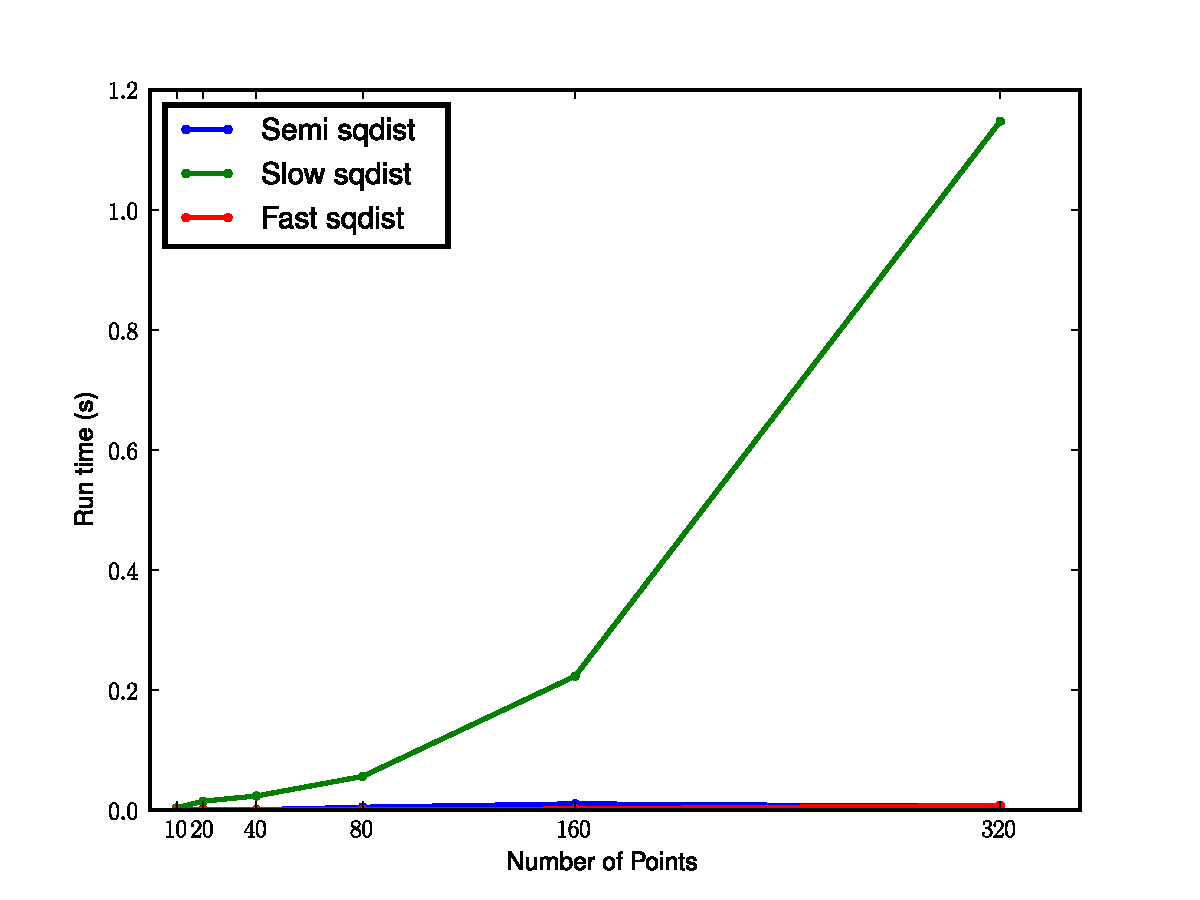
\includegraphics[width=\textwidth]{sqplot.pdf}
\caption{Runtimes of \li{sqdist} with varying degrees of vectorization.}
\label{fig:sqplot}
\end{figure}

Notice that often it is much easier to partially vectorize a calculation than it is to vectorize the entire calculation.
In many cases a partial vectorization will more than sufficient.  Vectorizing the inner loop was clearly worth the effort.

\section*{Shuffle}
This exercise is to write a program that shuffles a deck of a cards how a human would shuffle them, as opposed to having a random number generator put them in a random arrangement. 
In order to this, first, cut the deck in half. 
Say that either the top card in the first half goes down then the top card in the second half or vice-versa.
Which one comes first should be random.
Follow the same procedure for the rest of the cards in the two halves. 
The following is the code implemented using a loop.
\begin{lstlisting}
from random import randint
def shuffle(deck):
    size = deck.size
    newdeck = np.empty_like(deck)
    for i in xrange(size/2):
         if randint(0,1) == 0:
            newdeck[i*2] = deck[i]
            newdeck[i*2+1] = deck[size/2+i]
         else:
            newdeck[i*2] = deck[size/2+i]
            newdeck[i*2+1] = deck[i]
    return newdeck
\end{lstlisting}

\begin{problem}
Write a function that shuffles a deck the same way as the function above using only array operations.
\end{problem}

\section*{Image Editor}
An image is often represented as a 3D array where the first and second dimensions are the height and width respectively and the third dimension represents the intensity of each of three color channels: red, green, and blue.
The code below can be used to read and display images in Python.
\begin{lstlisting}
import matplotlib.pyplot as plt
img = plt.imread(<image-file>)
plt.imshow(img)
plt.show()
\end{lstlisting}

Matplotlib can read in PNG images on its own, otherwise it will read in images using the Python Image Library.
Depending on the format of the image, it may be read as an array of floating point values between 0 and 1 or it may be read as an array of integer values between 0 and 255.
In this lab we will assume the latter.

\begin{problem}
Write a function that edits an array representing an image.
Include options that allow you to  invert the image, change it to grayscale, or add a motion blur (definitions below). 
The function should take in a image, a parameter that tells how to modify the image, and a optional parameter for the motion blur.
It should then plot the image. 
\end{problem}

\begin{itemize}
\item Invert:
Every color value for every pixel is changed to its inverse value. For example, 0 becomes 255, 230 becomes 25, and 127 becomes 128.
Remember that the minimum color value is 0 and the maximum is 255.

\item Grayscale:
To convert an image to grayscale, each pixel’s color value is changed to the average of 
the pixel’s red, green, and blue value. For example, if the pixel values are:
Red: 225 Green: 30 Blue: 131, we convert the 

Grayscale conversion: $\frac{225 + 30 + 131}{3} = 128$ (using integer division)
Red: 128 Green: 128 Blue: 128

\item Motion Blur:
An additional parameter $n>0$ will be used for motion blur.
The value of each color of each pixel is the average of that color value for $n$ pixels (from 
the current pixel to $n-1$) horizontally. So pixel \li{[x,y,0]} would turn in to the average of
pixel \li{[x, y, 0]} to pixel \li{[x, y+n-1, 0]}.
Note: You will need to use one \li{for} loop here.
Be sure to account for the situations where one or more of the values used in the computing the average do not exist. For example, if an image has width $w$ and we are considering the pixel on row $r$, column $c$, if $c + n \geq w$, then we only average the pixels up to $w$. (Proper array slicing should take care of this case without any extra code.)

\end{itemize}

